% Adjust these for the path of the theme and its graphics, relative to this file
%\usepackage{beamerthemeFalmouthGamesAcademy}
\usepackage{../../beamerthemeFalmouthGamesAcademy}
\usepackage{multimedia}
\graphicspath{ {../../} }

% Default language for code listings
\lstset{language=C++,
        morekeywords={each,in,nullptr}
}

% For strikethrough effect
\usepackage[normalem]{ulem}
\usepackage{wasysym}
\usepackage{graphicx} %package to manage images

\usepackage{pdfpages}

% http://www.texample.net/tikz/examples/state-machine/
\usetikzlibrary{arrows,automata}

\newcommand{\modulecode}{COMP702}\newcommand{\moduletitle}{Classical Artificial Intelligence}\newcommand{\sessionnumber}{1}

\begin{document}
\title{\sessionnumber: Module Introduction}
\subtitle{\modulecode: \moduletitle}

\begin{frame}
	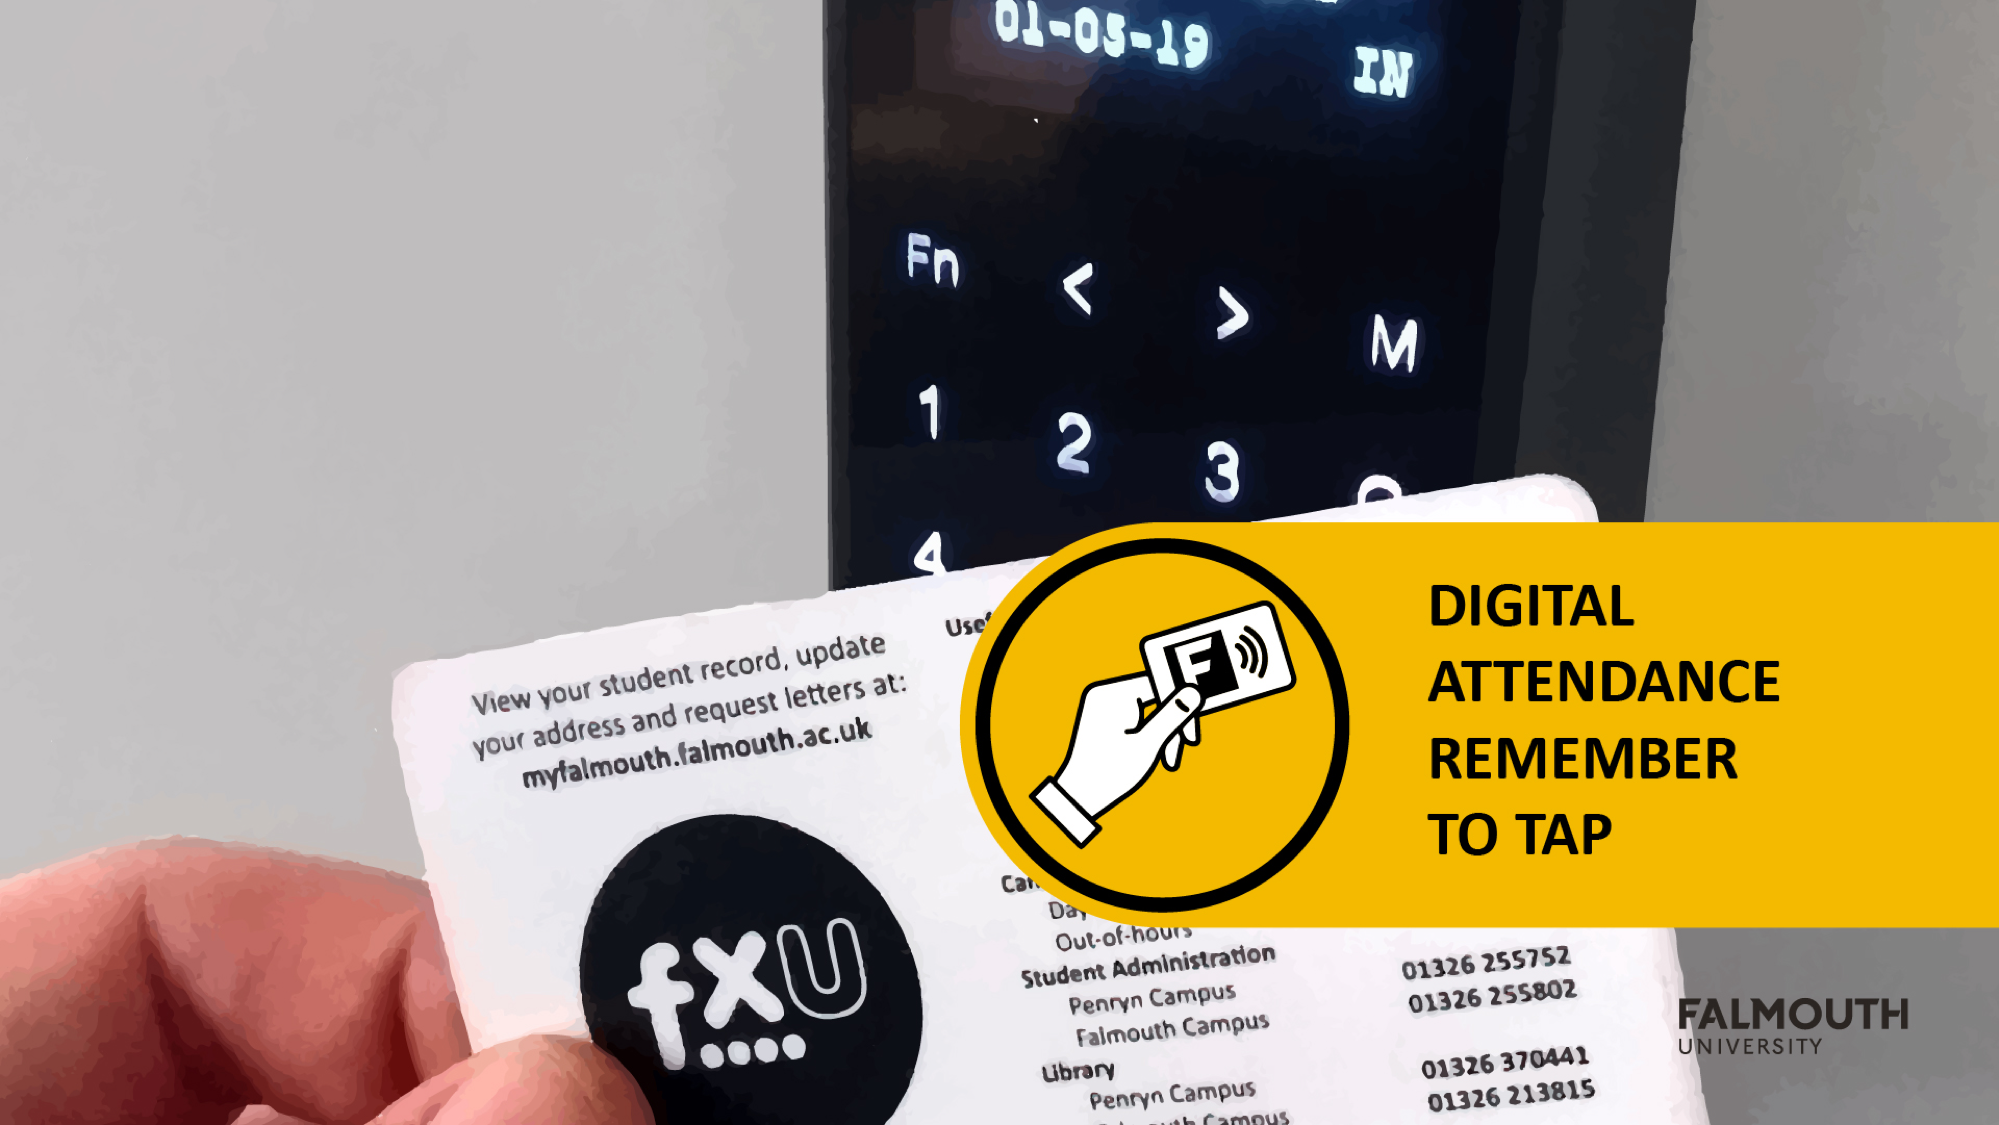
\includegraphics[width=1.0\textwidth]{sign-in}
\end{frame}

\frame{\titlepage} 



\begin{frame}
	\begin{columns}
		\column{0.5\textwidth}
		
\includegraphics[width=1.0\textwidth]{brian_mcdonald}
		\column{0.5\textwidth}
		\begin{itemize}
			\item Brian McDonald
			\item brian.mcdonald@falmouth.ac.uk
			\item Please contact me with any issues at all!
		\end{itemize}
	\end{columns}
\end{frame}

\begin{frame}{Today's agenda}
	\begin{itemize}
		\item GAM702 course outline
		\item GAM702 assignment
		\item First brief
	\end{itemize}
\end{frame}

\part{Module introduction}
\frame{\partpage}

\begin{frame}{Aim}
\begin{center}
To confidently implement artificial intelligence techniques which are commonly used to solve problems in industry.
\end{center}
\end{frame}

\begin{frame}{Description}
This module introduces you to the core techniques of artificial intelligence (AI): computational techniques for tackling problems that normally require human intelligence. You will refine your understanding of these techniques by applying them to well-defined problem domains, laying the foundation for more complex applications in subsequent modules. A deep knowledge of the past and present of AI will equip you for future developments in this fast-moving field.
\end{frame}

\begin{frame}{Description (cont)}
This module covers ``classical'' AI focusing upon techniques that are commonly applied to decision-making and content generation in games and beyond. Applications of such techniques include the authoring of non-player character behaviours in games, the navigation of complex environments, the formation of logistical plans with respect to constraints, and the generation of content in creative domains. You will build a portfolio of AI instances applied to simplified versions of these and other domains. Thus you will study the strengths and weaknesses of standard AI techniques, gaining the ability to select appropriate technologies to solve real problems and to contextualise recent advances in the field.
\end{frame}

\begin{frame}{Assignments}
	\begin{itemize}
		\pause\item Assignment 1: Portfolio of AI Instances (100\%)
		\pause\item A portfolio of \textbf{three} AI demos
		    \begin{itemize}
		        \item Authored behaviours
		        \item Search / planning
		        \item Logic programming / constraint solving
		    \end{itemize}
		\pause\item See LearningSpace for assignment brief
		\pause\item See MyFalmouth for deadline
	\end{itemize}
\end{frame}

\begin{frame}{Timetable}
	\begin{itemize}
		\pause\item See MyTimetable
		\pause\item Weekly \textbf{lectures} (1hr) --- taught content
		\pause\item Weekly \textbf{workshops} (2hr) --- development support
		\pause\item Fortnightly \textbf{seminars} (2hr) --- paper discussion
	\end{itemize}
\end{frame}

\begin{frame}{Paper Club}
    Please read the following paper ahead of next week's seminar:
    
    Shoulson A., Garcia F.M., Jones M., Mead R., Badler N.I. (2011) Parameterizing Behavior Trees. In: Allbeck J.M., Faloutsos P. (eds) Motion in Games. MIG 2011. Lecture Notes in Computer Science, vol 7060. Springer, Berlin, Heidelberg
    
    (See LearningSpace for PDF link)
\end{frame}


\part{Resources}
\frame{\partpage}

\part{Game Engines}
\frame{\partpage}

\begin{frame}{Unity}
	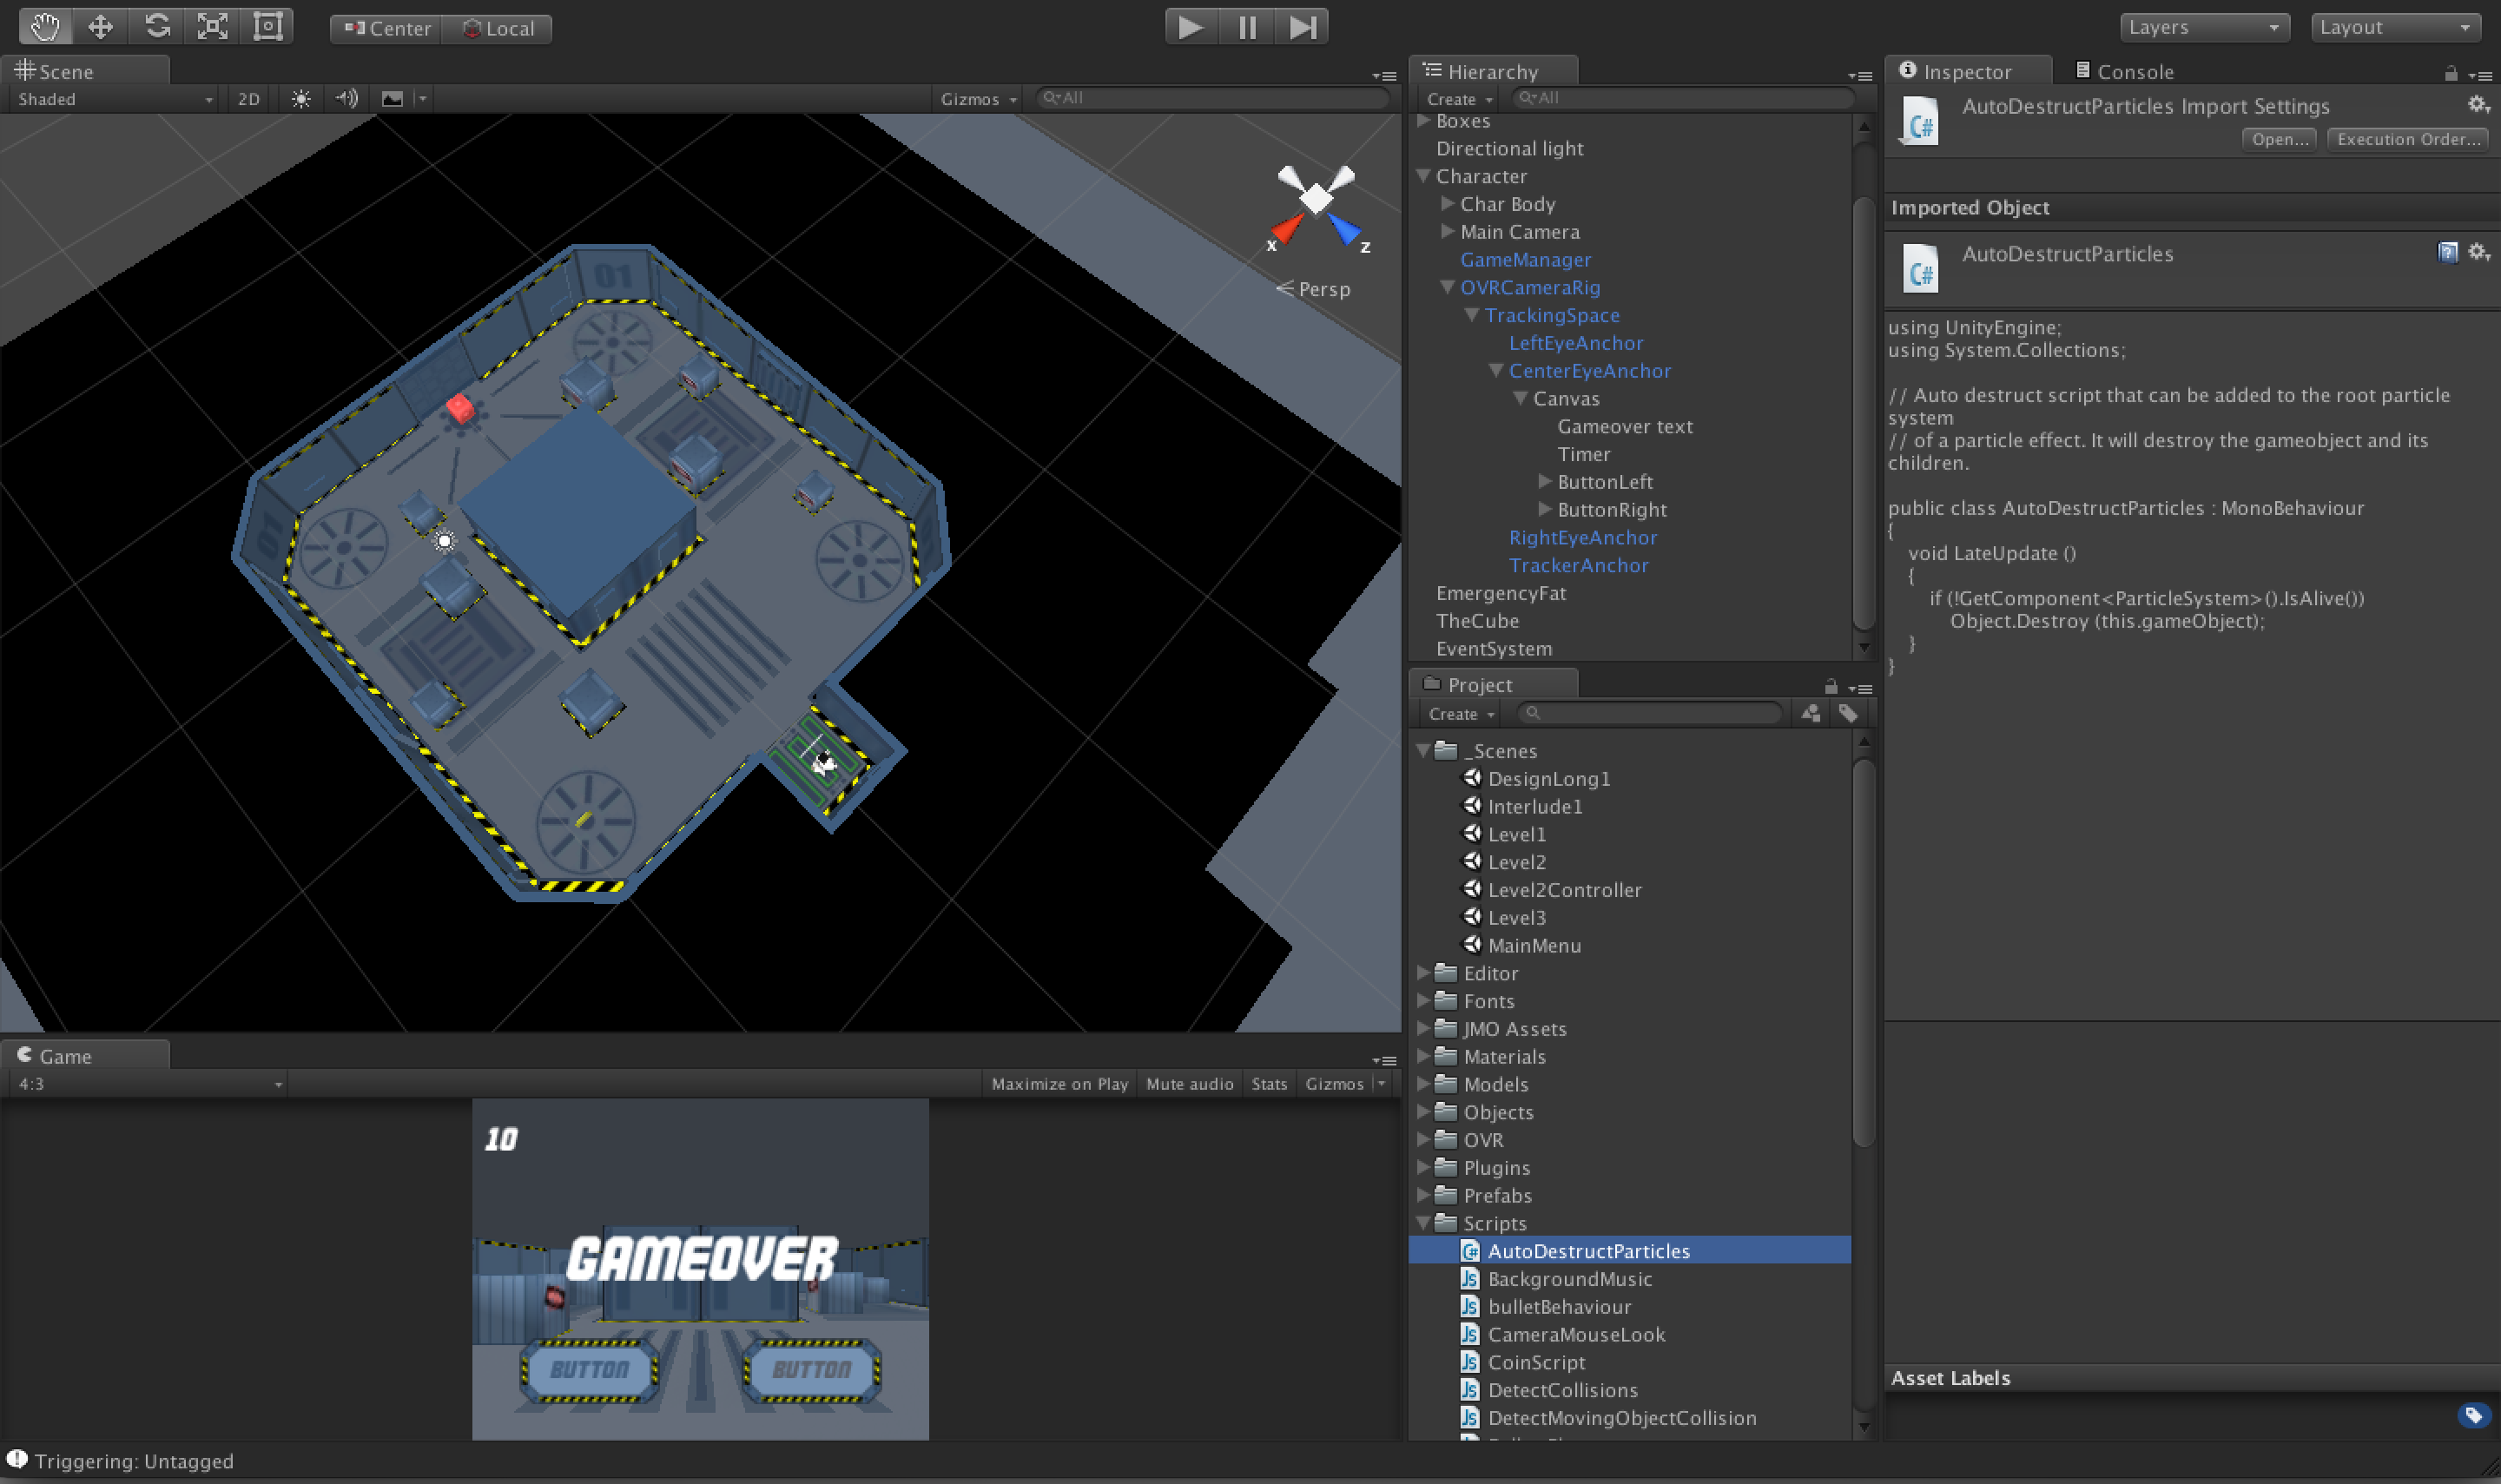
\includegraphics[width=1.0\textwidth]{unity}
\end{frame}

\begin{frame}{UE4}
	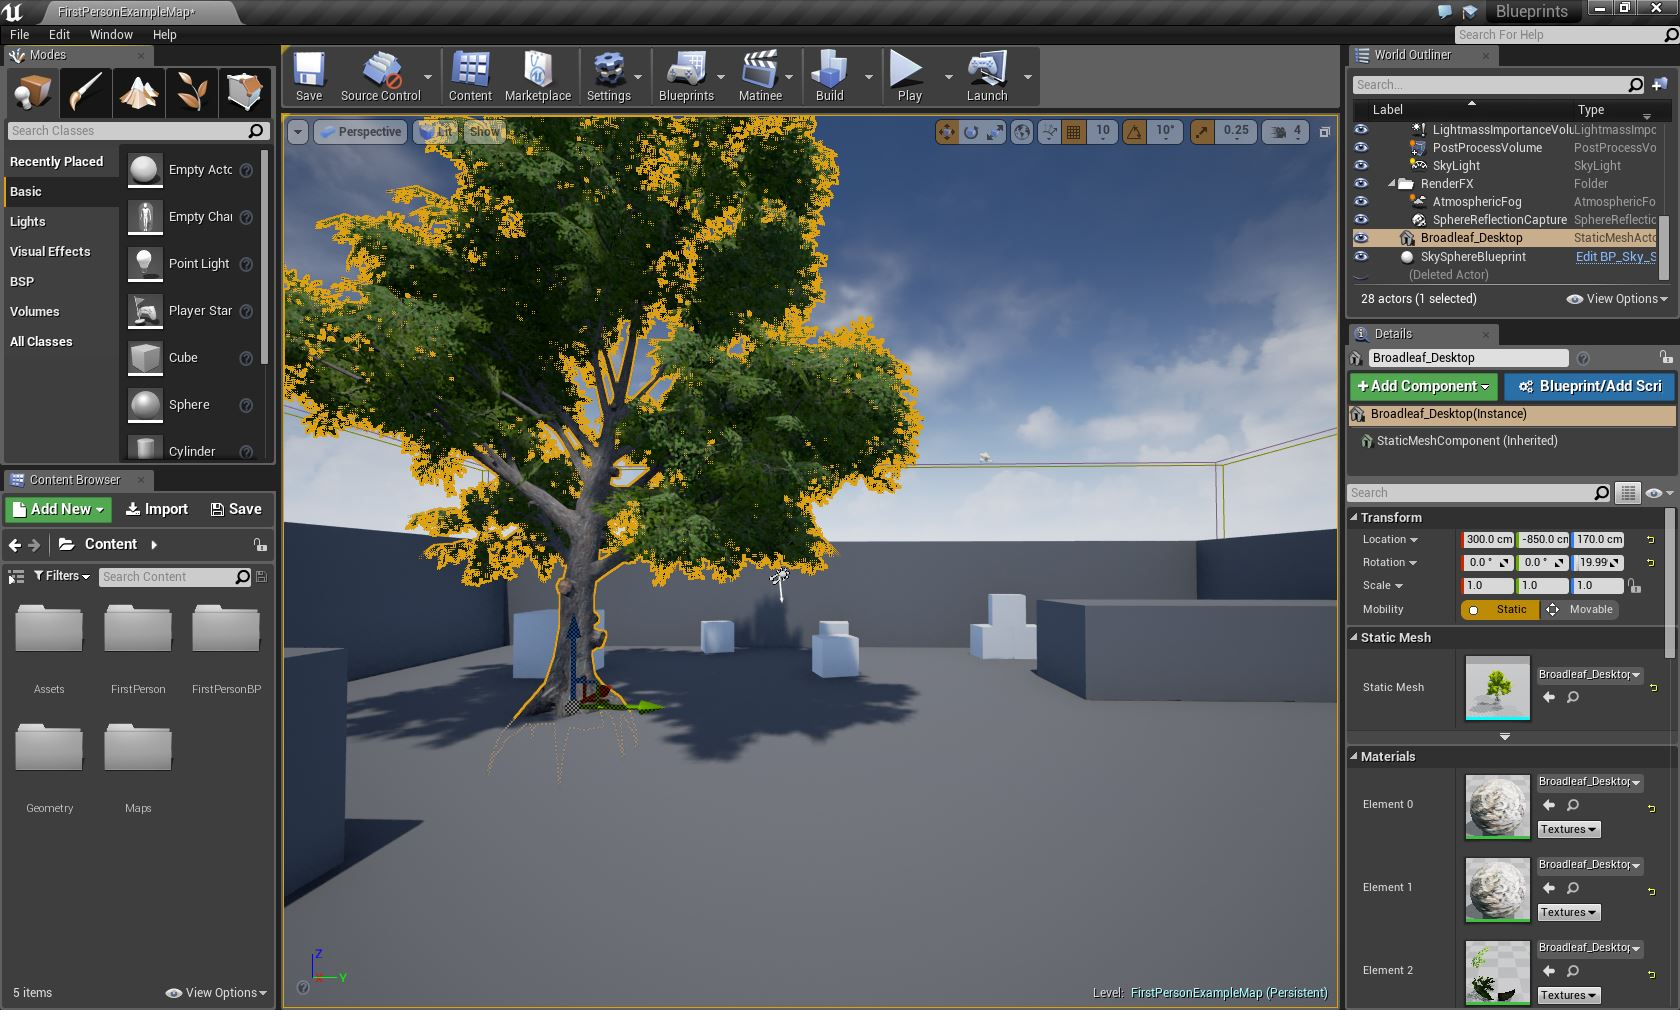
\includegraphics[width=1.0\textwidth]{ue4}
\end{frame}

\begin{frame}{Construct 2}
	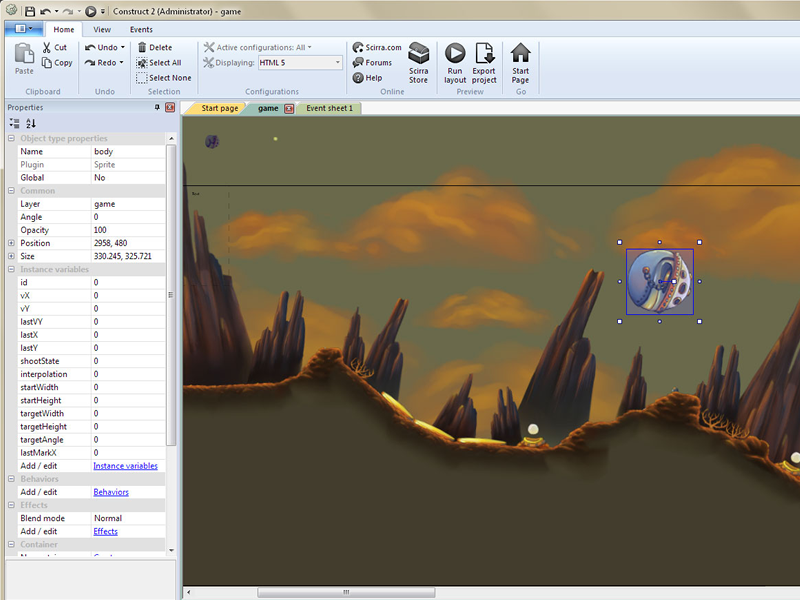
\includegraphics[width=0.9\textwidth]{construct2}
\end{frame}

\begin{frame}{Stencyl}
	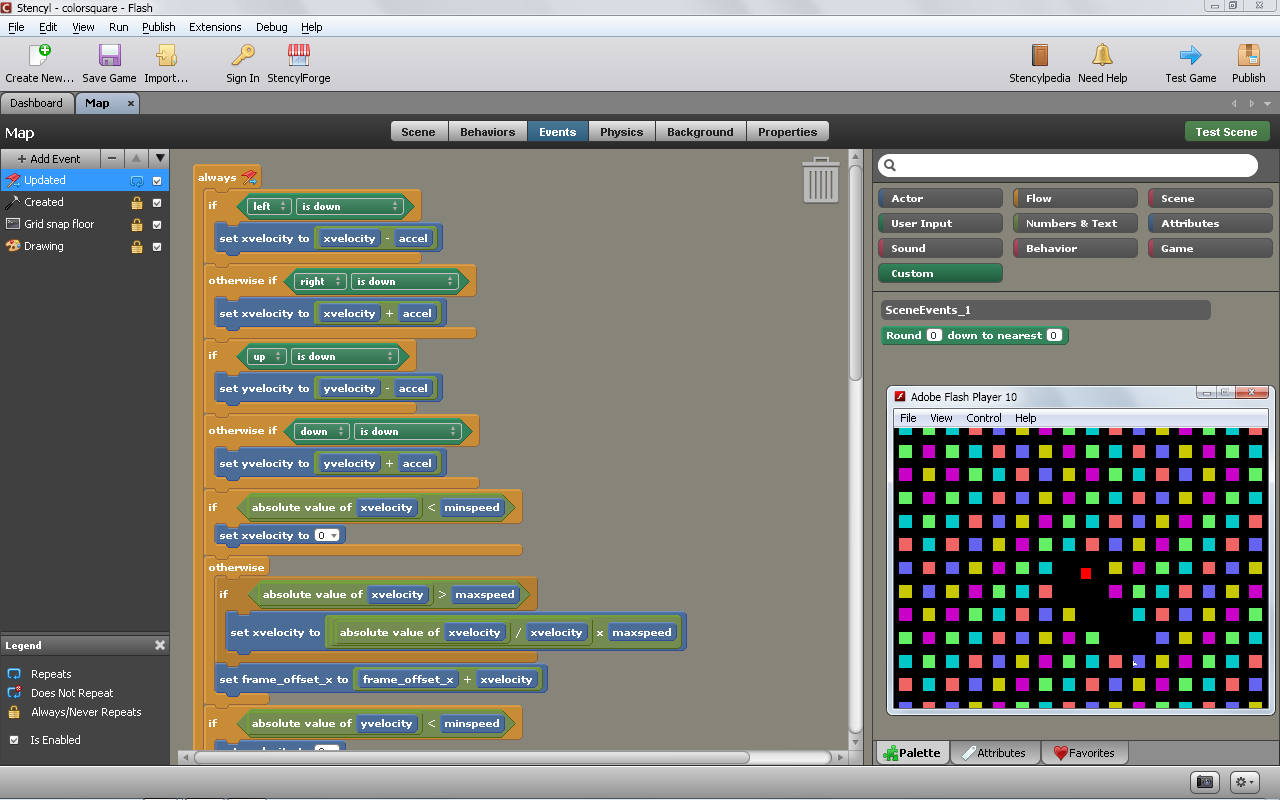
\includegraphics[width=1.0\textwidth]{stencyl}
\end{frame}

\begin{frame}{Gamemaker 2}
	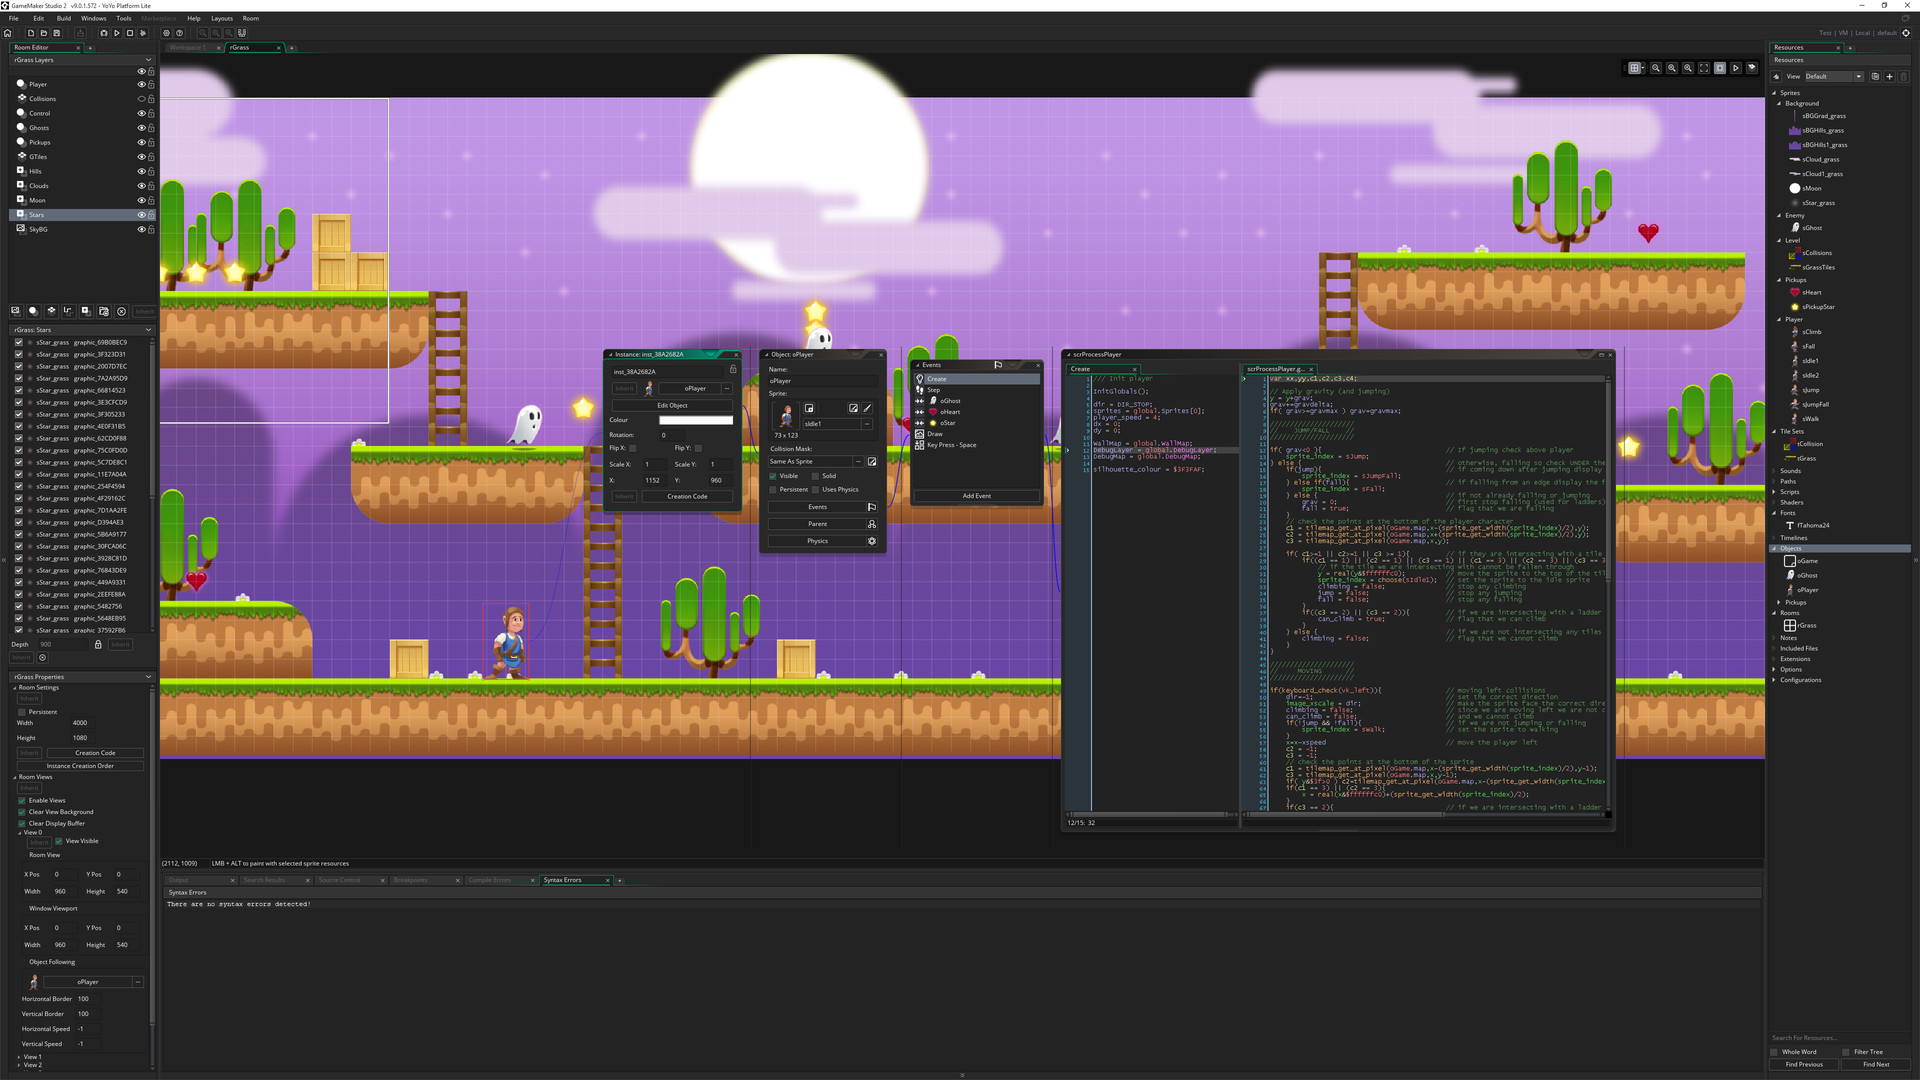
\includegraphics[width=1.0\textwidth]{gamemaker2}
\end{frame}
\part{Other Digital Options}
\frame{\partpage}

\begin{frame}
	\begin{itemize}
		\item Bitsy
		\item Twine
		\item Inkle
		\item Unity with Fungus
		\item Renpy
		\item Flat Games
	\end{itemize}
\end{frame}

\begin{frame}{Bitsy}
	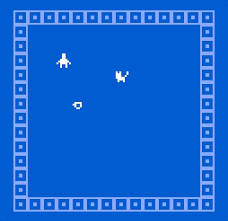
\includegraphics[width=1.0\textwidth, height=0.7\textheight]{bitsy}
\end{frame}

\begin{frame}{Twine}
	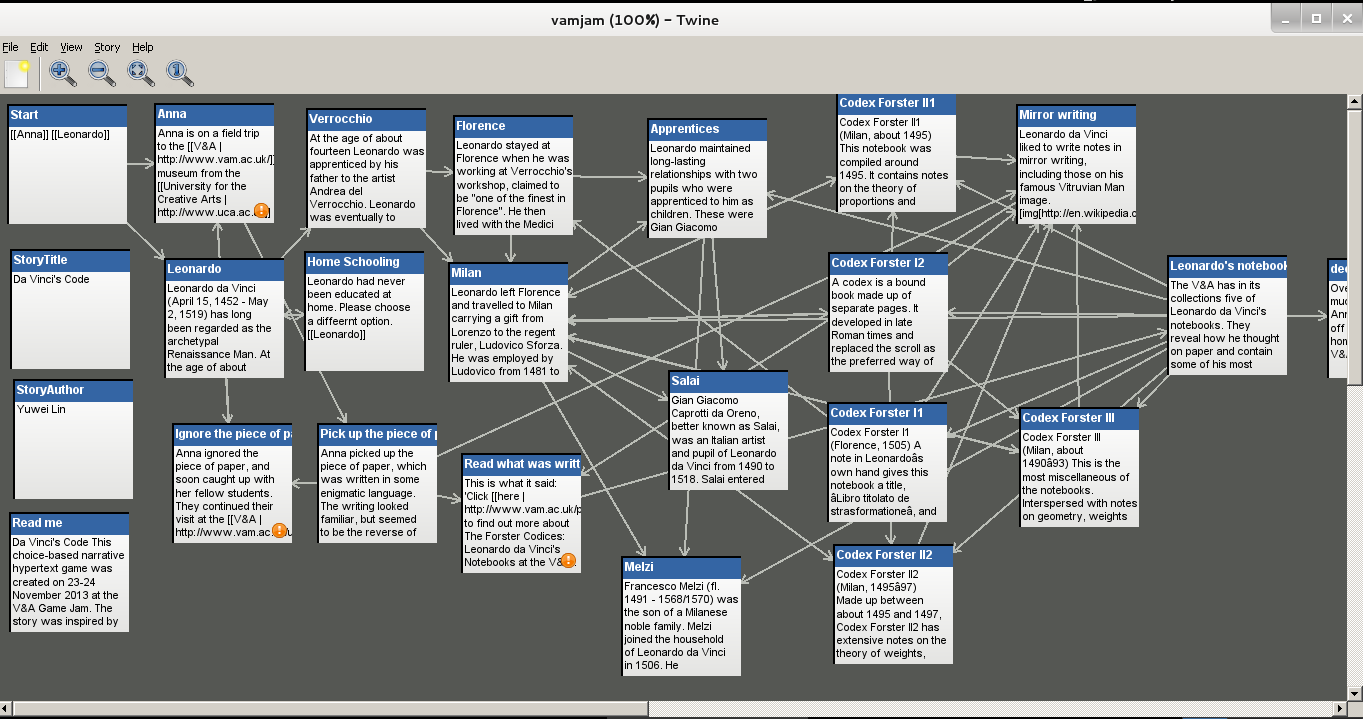
\includegraphics[width=1.0\textwidth]{twine}
\end{frame}

\begin{frame}{Inkle}
	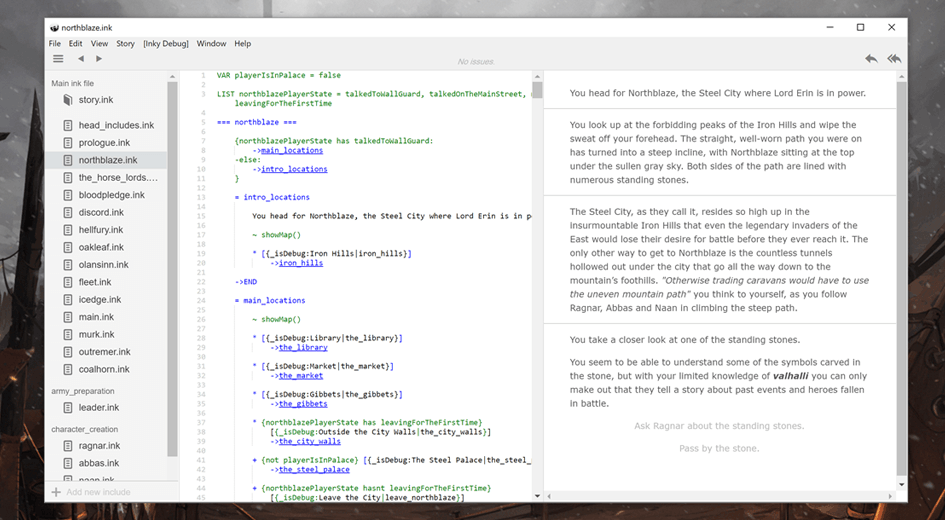
\includegraphics[width=1.0\textwidth]{inkle}
\end{frame}

\begin{frame}{Unity with Fungus}
	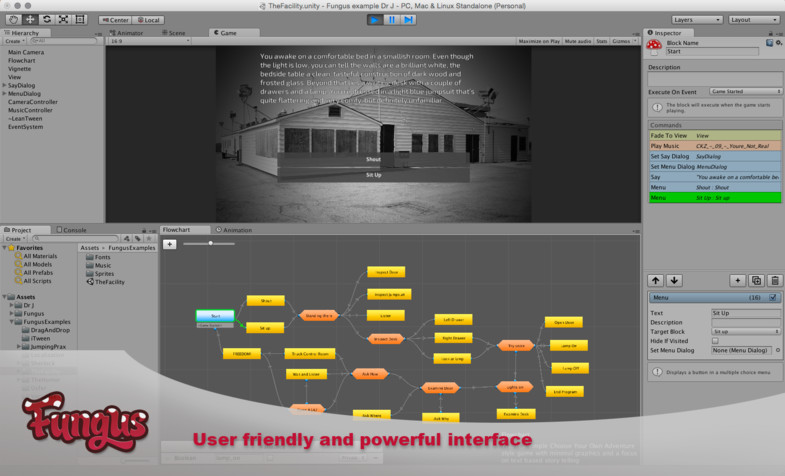
\includegraphics[width=1.0\textwidth]{fungus}
\end{frame}

\begin{frame}{Renpy}
	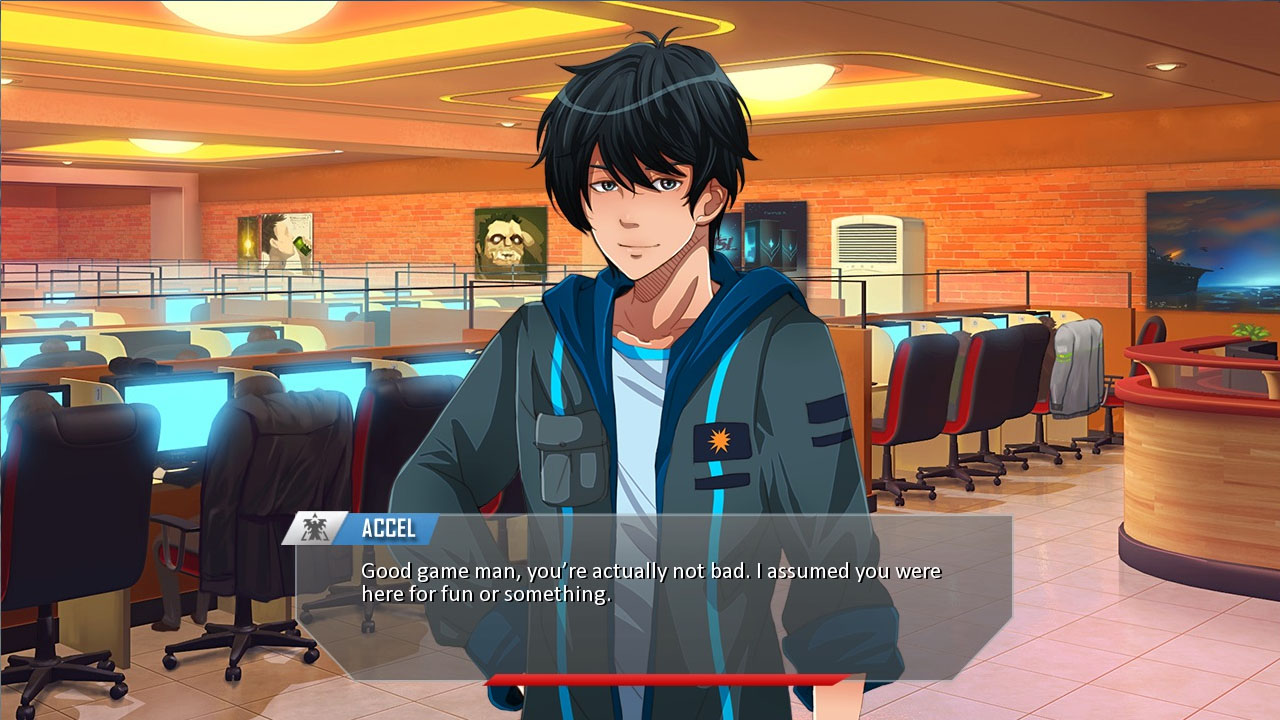
\includegraphics[width=1.0\textwidth]{renpy}
\end{frame}

\begin{frame}{Flat Games}
	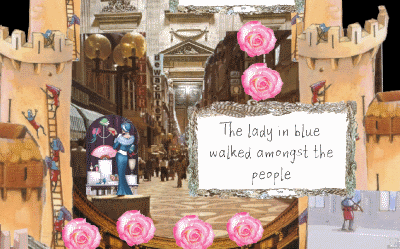
\includegraphics[width=1.0\textwidth]{flat_games}
\end{frame}
\part{Physical Games}
\frame{\partpage}

\begin{frame}{Board \& Cardgames}
	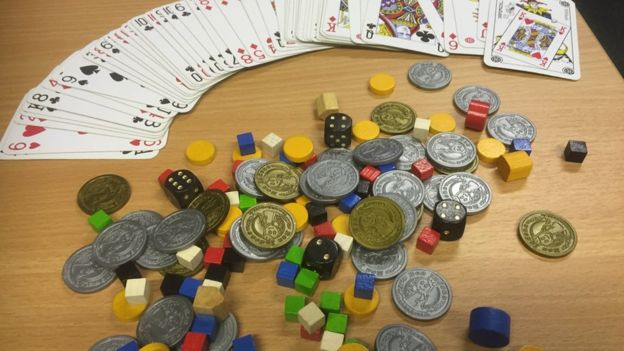
\includegraphics[width=1.0\textwidth]{card_boardgames}
\end{frame}

\begin{frame}{Board \& Cardgames}
	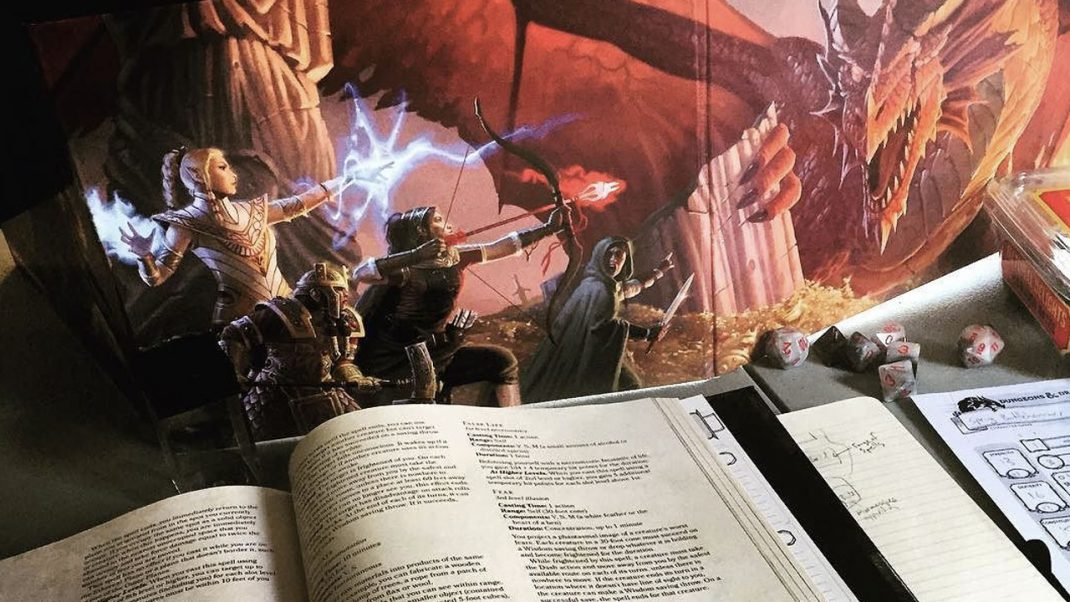
\includegraphics[width=1.0\textwidth]{rpg_campaign}
\end{frame}

\begin{frame}{Playground Games}
	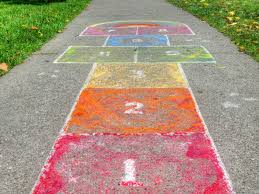
\includegraphics[width=1.0\textwidth, height=0.7\textheight]{hop_scotch}
\end{frame}

\begin{frame}{Traditional or Folk Games}
	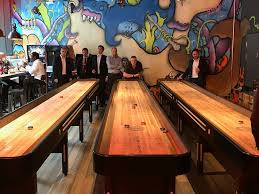
\includegraphics[width=1.0\textwidth, height=0.7\textheight]{shuffle_board}
\end{frame}






\begin{frame}{First Prototype - Theme Announcement}
	\url{http://youtube.com}
\end{frame}

\end{document}
